\chapter{Introduction} % Main chapter title
\label{chap:Chapter1}  % For referencing this chapter elsewhere, use \ref{Chapter1}
\epigraph{``Alone we can do so little, together we can do so much” }{\textit{Hellen Keller}}


Τα τελευταία χρόνια η ανάπτυξη της επιστήμης έχει επιφέρει την απόκτηση των τεχνολογικών επιτευγμάτων 
από το ευρύ κοινό\udot με ένα πολύ οικονομικό αντίτιμο. Αυτό σημαίνει ότι ο καθένας πολύ εύκολα, μπορεί 
να έχει στην κατοχή του ακόμα και προϊόντα τα οποία θεωρούνται state-of-the-art, χωρίς να χρειάζεται να 
δαπανήσει μεγάλα ποσά. Το ίδιο φυσικά συμβαίνει και με τον κλάδο των drone και την - κατά επέκταση - χρήση 
αυτών\udot ακόμα και για ψυχαγωγικό σκοπό.  

Κατά το τέλος του έτους 2019 μόνο στις Ηνωμένες Πολιτείες της Αμερικής υπήρχαν πάνω από 990 χιλιάδες 
εγγεγραμμένοι χειριστές drone με πάνω από 1.32 εκατομμύρια drone ψυχαγωγικού χαρακτήρα να χρησιμοποιούνται 
\cite{2019-drone-statistic}. Ενώ μέχρι το 2025 υπολογίζεται ότι το μέγεθος αγοράς των υπηρεσιών drone θα 
κοστολογείται στα 63.6 δισεκατομμύρια δολάρια \cite{expected-drone-market}.

Φυσικά η χρήση τους δεν περιορίζεται μόνο στην ψυχαγωγία, εταιρίες όπως η Amazon έχουν αποκτήσει ήδη τα 
απαραίτητα πιστοποιητικά και εγκρίσεις, με σκοπό να χρησιμοποιήσουν drone για παράδοση των δεμάτων αρκετά 
σύντομα \cite{amazon-drones}, καθώς προς το παρόν η διαδικασία βρίσκεται σε στάδιο δοκιμών. Συνεπώς είναι 
εύκολο να κατανοηθεί ότι ο συγκεκριμένος κλάδος πρόκειται να έχει ακόμα μεγαλύτερη άνθιση, με αρκετά μεγάλο 
ερευνητικό ενδιαφέρον να του αναλογεί.   

Με την αύξηση των drone και την αύξηση των εφαρμογών, υπάρχει η ανάγκη συνε\-ργασίας και η δημιουργία drone swarms 
για την επιτυχή ολοκλήρωση των στόχων που έχουν οριστεί. Όμως για να καταφέρουν τα drone να συνεργαστούν, χρειάζεται 
πρώτα να μπορούν να ξεπεράσουν τα προβλήματα τα οποία υπάρχουν. Με ένα από τα μεγαλύτερα να είναι η πλήρη γνώση της 
θέσης τους στον χώρο.

\newpage

%----------------------------------------------------------------------------------------
%	SECTION 1
%----------------------------------------------------------------------------------------
\section{Unmanned aerial vehicles} \label{sec:Chapter1-1} 

Είναι σημαντικό από τα πρώτα βήματα, να έχει γίνει κατανοητό με τον όρο drone σε τι παραπέμπουμε - όπως επίσης πότε 
θεωρείται ότι ένα σμήνος από drone πετάει σε σχηματισμό (drone swarm).

%----------------------------------------------------------------------------------------
\subsection{History and drone types} \label{sec:Chapter1-1-1}
Όταν αναφερόμαστε στον όρο Unmanned Aerial Vehicle (\Abbr{UAV}) ή απλούστερα drone κάνουμε αναφορά για ένα μη επανδρωμένο 
ιπτάμενο αεροσκάφος το οποίο ελέγχεται είτε απομακρυσμένα από έναν άνθρωπο, είτε είναι τελείως αυτόνομο. Τα \Abbr{UAV} μαζί 
με ένα Base Station (\Abbr{BS}) και την από κοινού επικοινωνίας του σταθμού - drone, δημιουργούν αυτό που ονομάζουμε Unmanned 
Aircraft System (\Abbr{UAS}) \cite{what-is-UAV} \cite{what-is-UAV-and-history}.

Η πρώτη εμφάνιση των \Abbr{UAV} έγινε κατά το 1849 στα πλαίσια μάχης, ενώ οι πρώτες καινοτομίες πάνω σε αυτά ξεκίνησαν ήδη από 
τις αρχές του 20ου αιώνα. Το 2013 τουλάχιστον 50 χώρες χρησιμοποιούσαν \Abbr{UAV}<s> για κάποιον σκοπό, με μερικές από αυτές 
φυσικά να σχεδιάζουν τα δικά τους \cite{what-is-UAV-and-history}. Αυτήν την στιγμή υπάρχουν πάνω από 1000 διαφορετικά μοντέλα 
\Abbr{UAV} που χρησιμοποιούνται ανά τον κόσμο, με τα περισσότερα από αυτά να μην έχουν ψυχαγωγικό χαρακτήρα \cite{list-of-UAVs}. 

Είναι λοιπόν ξεκάθαρο ότι το πλήθος των drone είναι τόσο μεγάλο, λόγω των δια\-φορετικών αναγκών - και ότι κάποια έχουν καλύτερα
αποτελέσματα από ότι άλλα σε συγκεκριμένες αποστολές. Για αυτό, έχουν γίνει ήδη προσπάθειες για την κατηγοριοποίηση των \Abbr{UAV}<s> 
σύμφωνα με τα διάφορα χαρακτηριστικά που μπορεί να έχουν. Ενδεικτικά με βάση το μέγεθος, την αυτονομία, το βάρος ή το μηχανολογικό 
σχεδια\-σμό των \Abbr{UAV} να είναι μερικές από τις υπάρχουσες \cite{what-is-UAV} \cite{drone-classification} 
\cite{application-areas|swarm-types|uavs-classification|sensor's-used|swarms-problems|public-awareness}.
Στο \Tabl{drone-determined-by-their-structure} υπά\-ρχει μία απλουστευμένη κατηγοριοποίηση η οποία προτάθηκε από τους συγγραφείς του 
\cite{application-areas|swarm-types|uavs-classification|sensor's-used|swarms-problems|public-awareness} σύμφωνα με τη βασική 
μηχανολογική δομή που μπορεί να έχει ένα drone καθώς και τα πλεονεκτήματα της κάθε δομής. 

% TABLE
\begin{table}[H]
    \caption[Classification of UAVs based on their structure]{Classification of  \Abbr{UAV}<s> based on their structure \cite{application-areas|swarm-types|uavs-classification|sensor's-used|swarms-problems|public-awareness}.}
    \label{tab:drone-determined-by-their-structure}
    \centering
    \begin{tabular}{ll}
        \toprule
        \textbf{Drones} & \textbf{Main features}  \\
        \midrule
            Fixed-Wing & long endurance and fast flight speed \\
            Fixed-Wing Hybrid & \Abbr{VTOL} and long endurance flight \\
            Single Rotor & \Abbr{VTOL}, hover, and long endurance flight \\
            Multirotor & \Abbr{VTOL}, hover, and short endurance flight \\
        \bottomrule
    \end{tabular}
\end{table}

% IMAGE
\begin{figure} [H]
    \centering
    % -----------------
    \begin{minipage}{.5\textwidth}
      \centering
      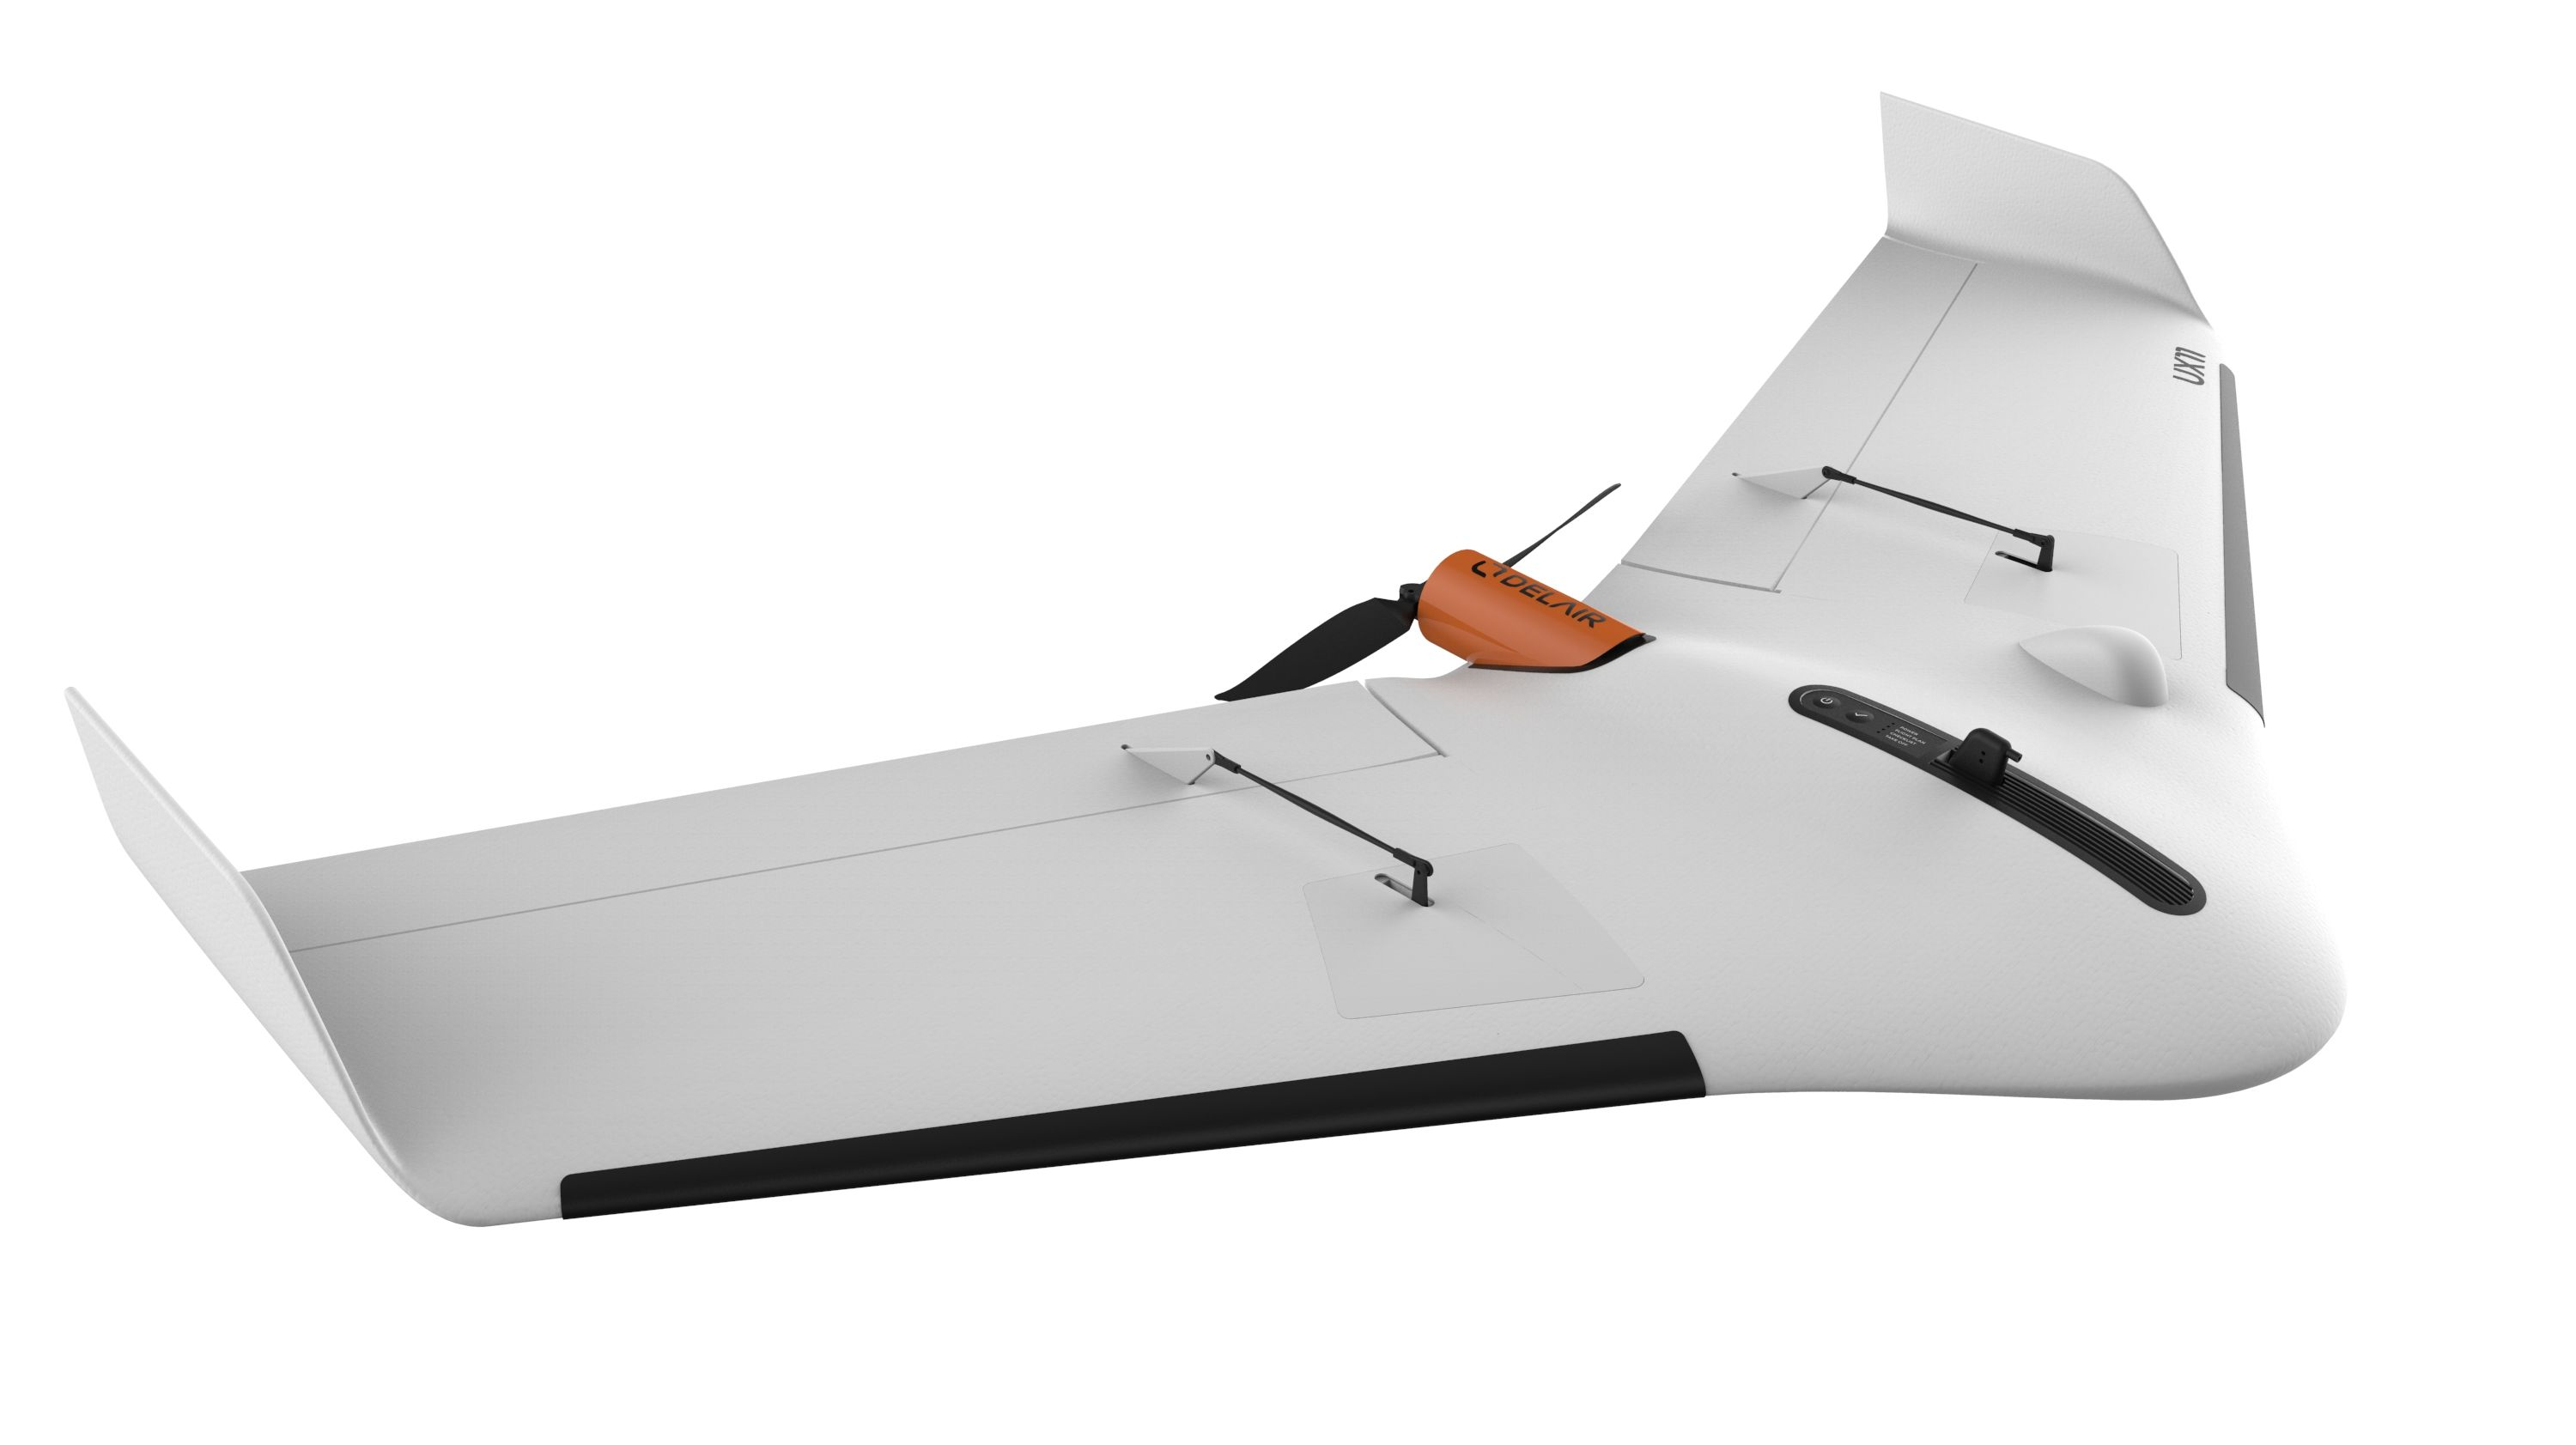
\includegraphics[width=\linewidth]{Images/Introduction/uav-fixed-wing-example.jpg}
      {(a) Fixed-Wing} \URI{https://delair.aero/portfolio/surveying-and-mapping/}
    \end{minipage}%
    % -----------------
    \begin{minipage}{.5\textwidth}
      \centering
      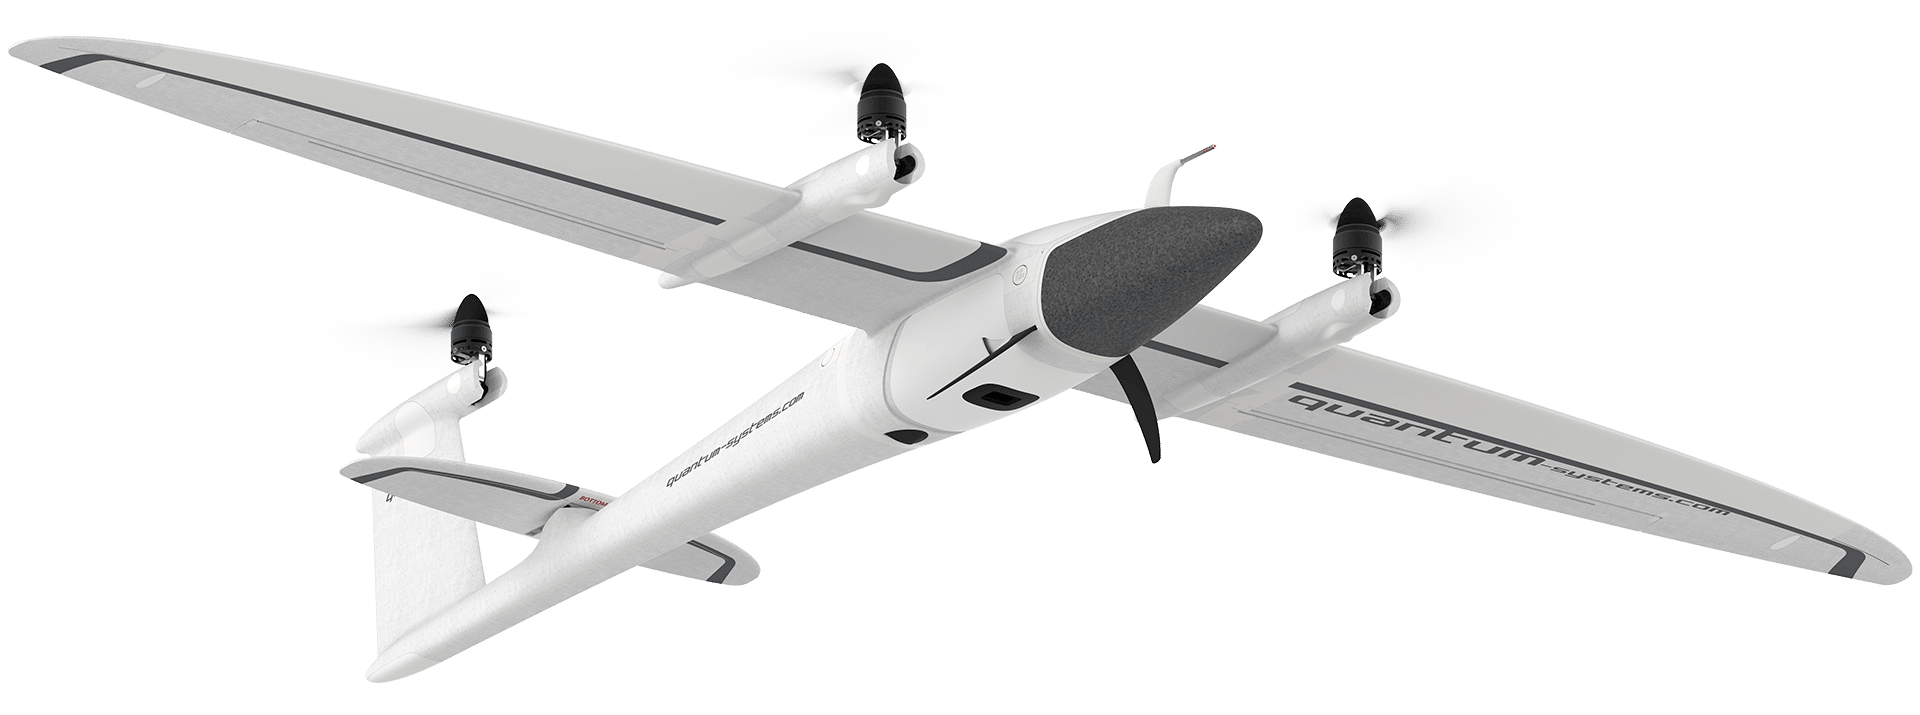
\includegraphics[width=\linewidth]{Images/Introduction/uav-fixed-wing-hybrid-example.png}
      {(b) Fixed-Wing Hybrid} \URI{https://www.quantum-systems.com/project/trinity-f90/}
    \end{minipage}
    % -----------------
    \begin{minipage}{.5\textwidth}
        \centering
        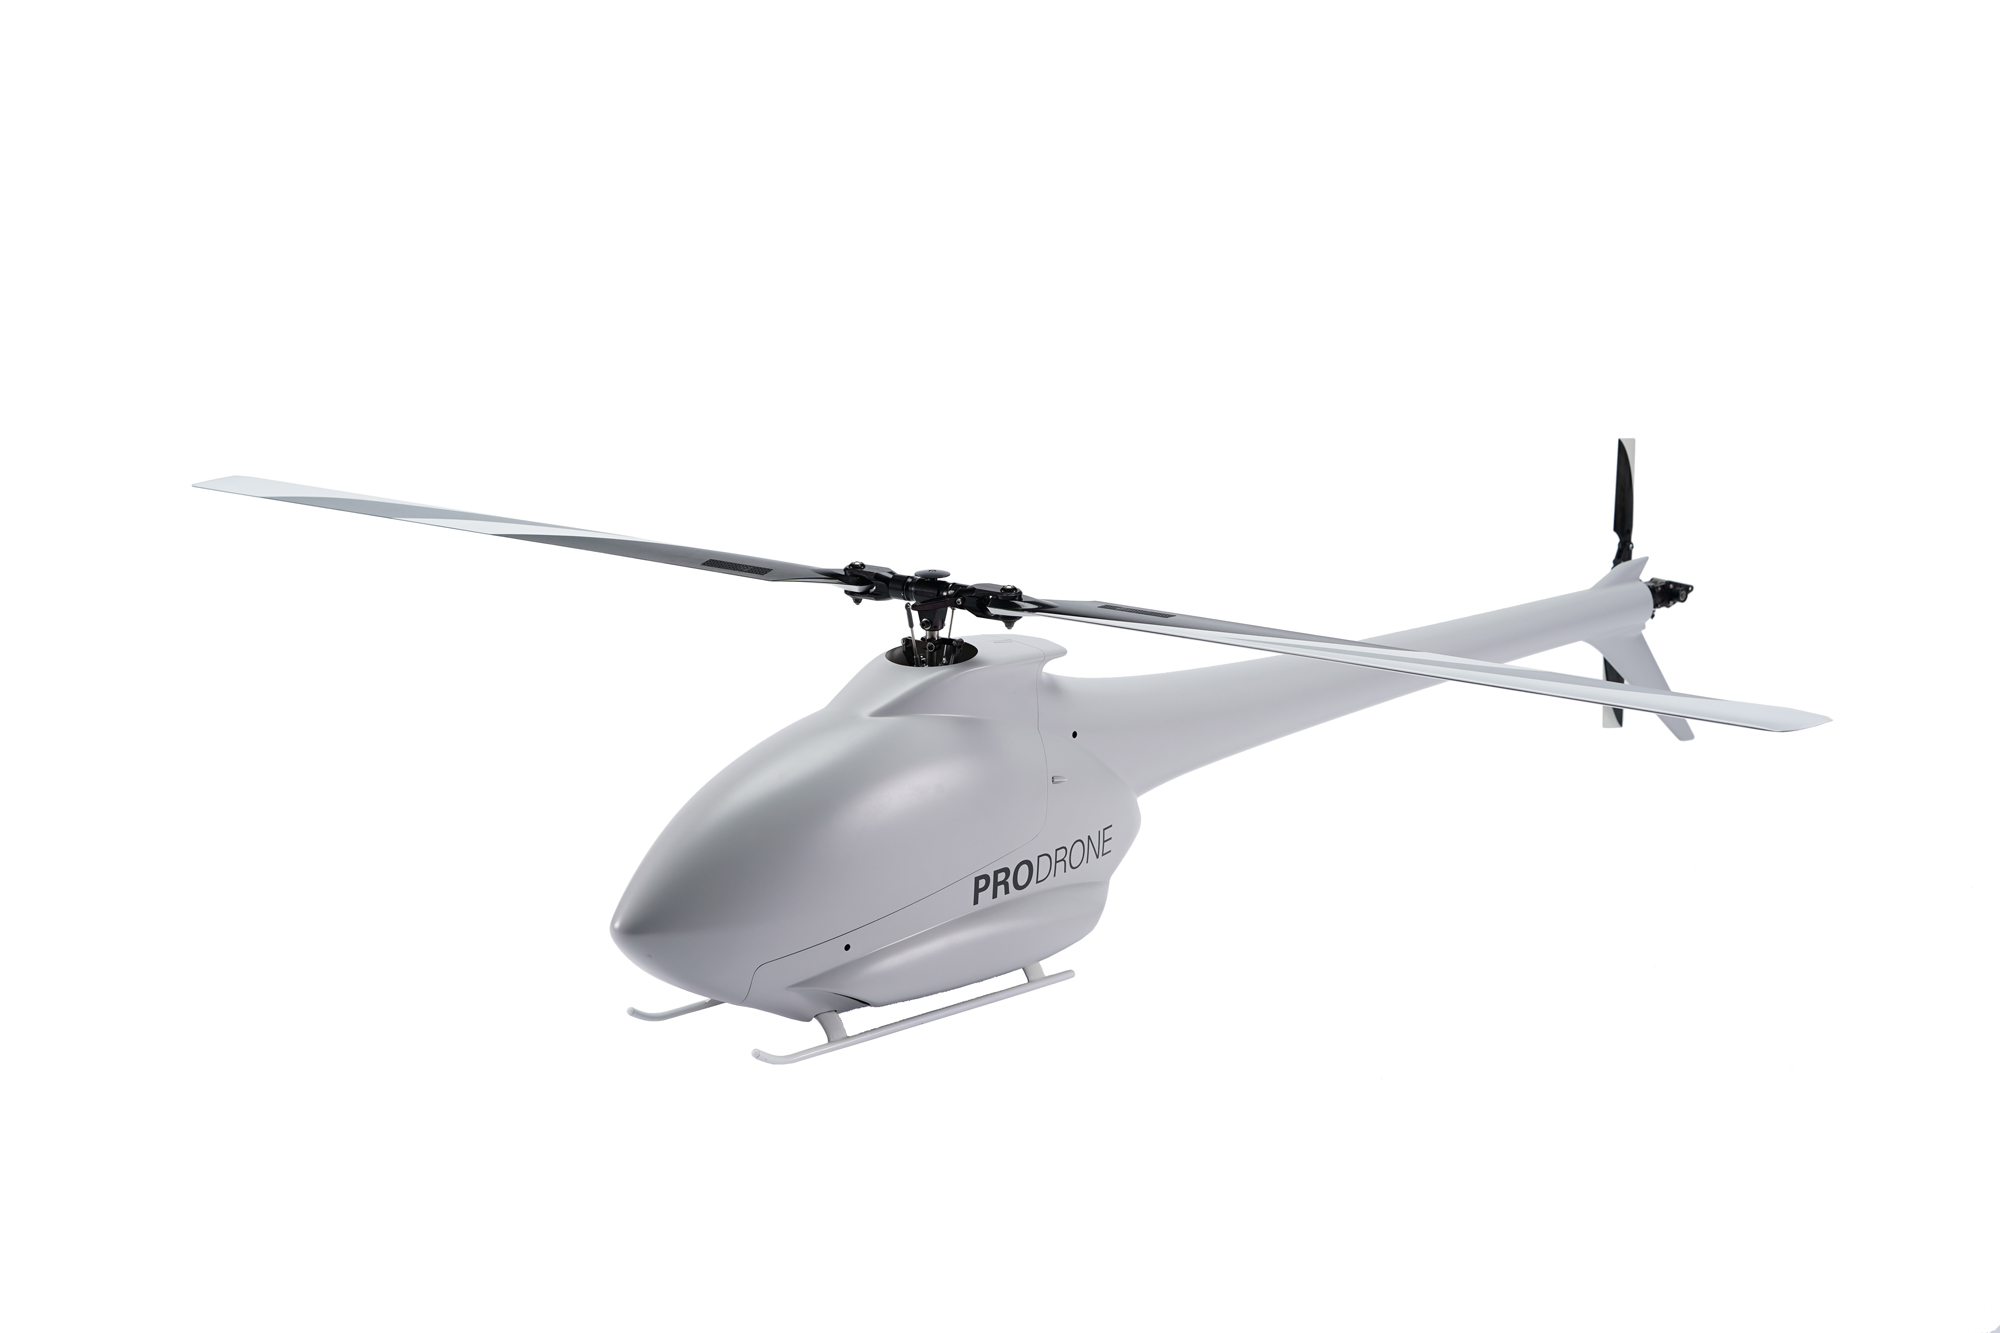
\includegraphics[width=\linewidth]{Images/Introduction/uav-single-rotor-example.jpg}
        {(c) Single Rotor} \URI{https://www.prodrone.com/release-en/2874/}
      \end{minipage}%
      % -----------------
      \begin{minipage}{.5\textwidth}
        \centering
        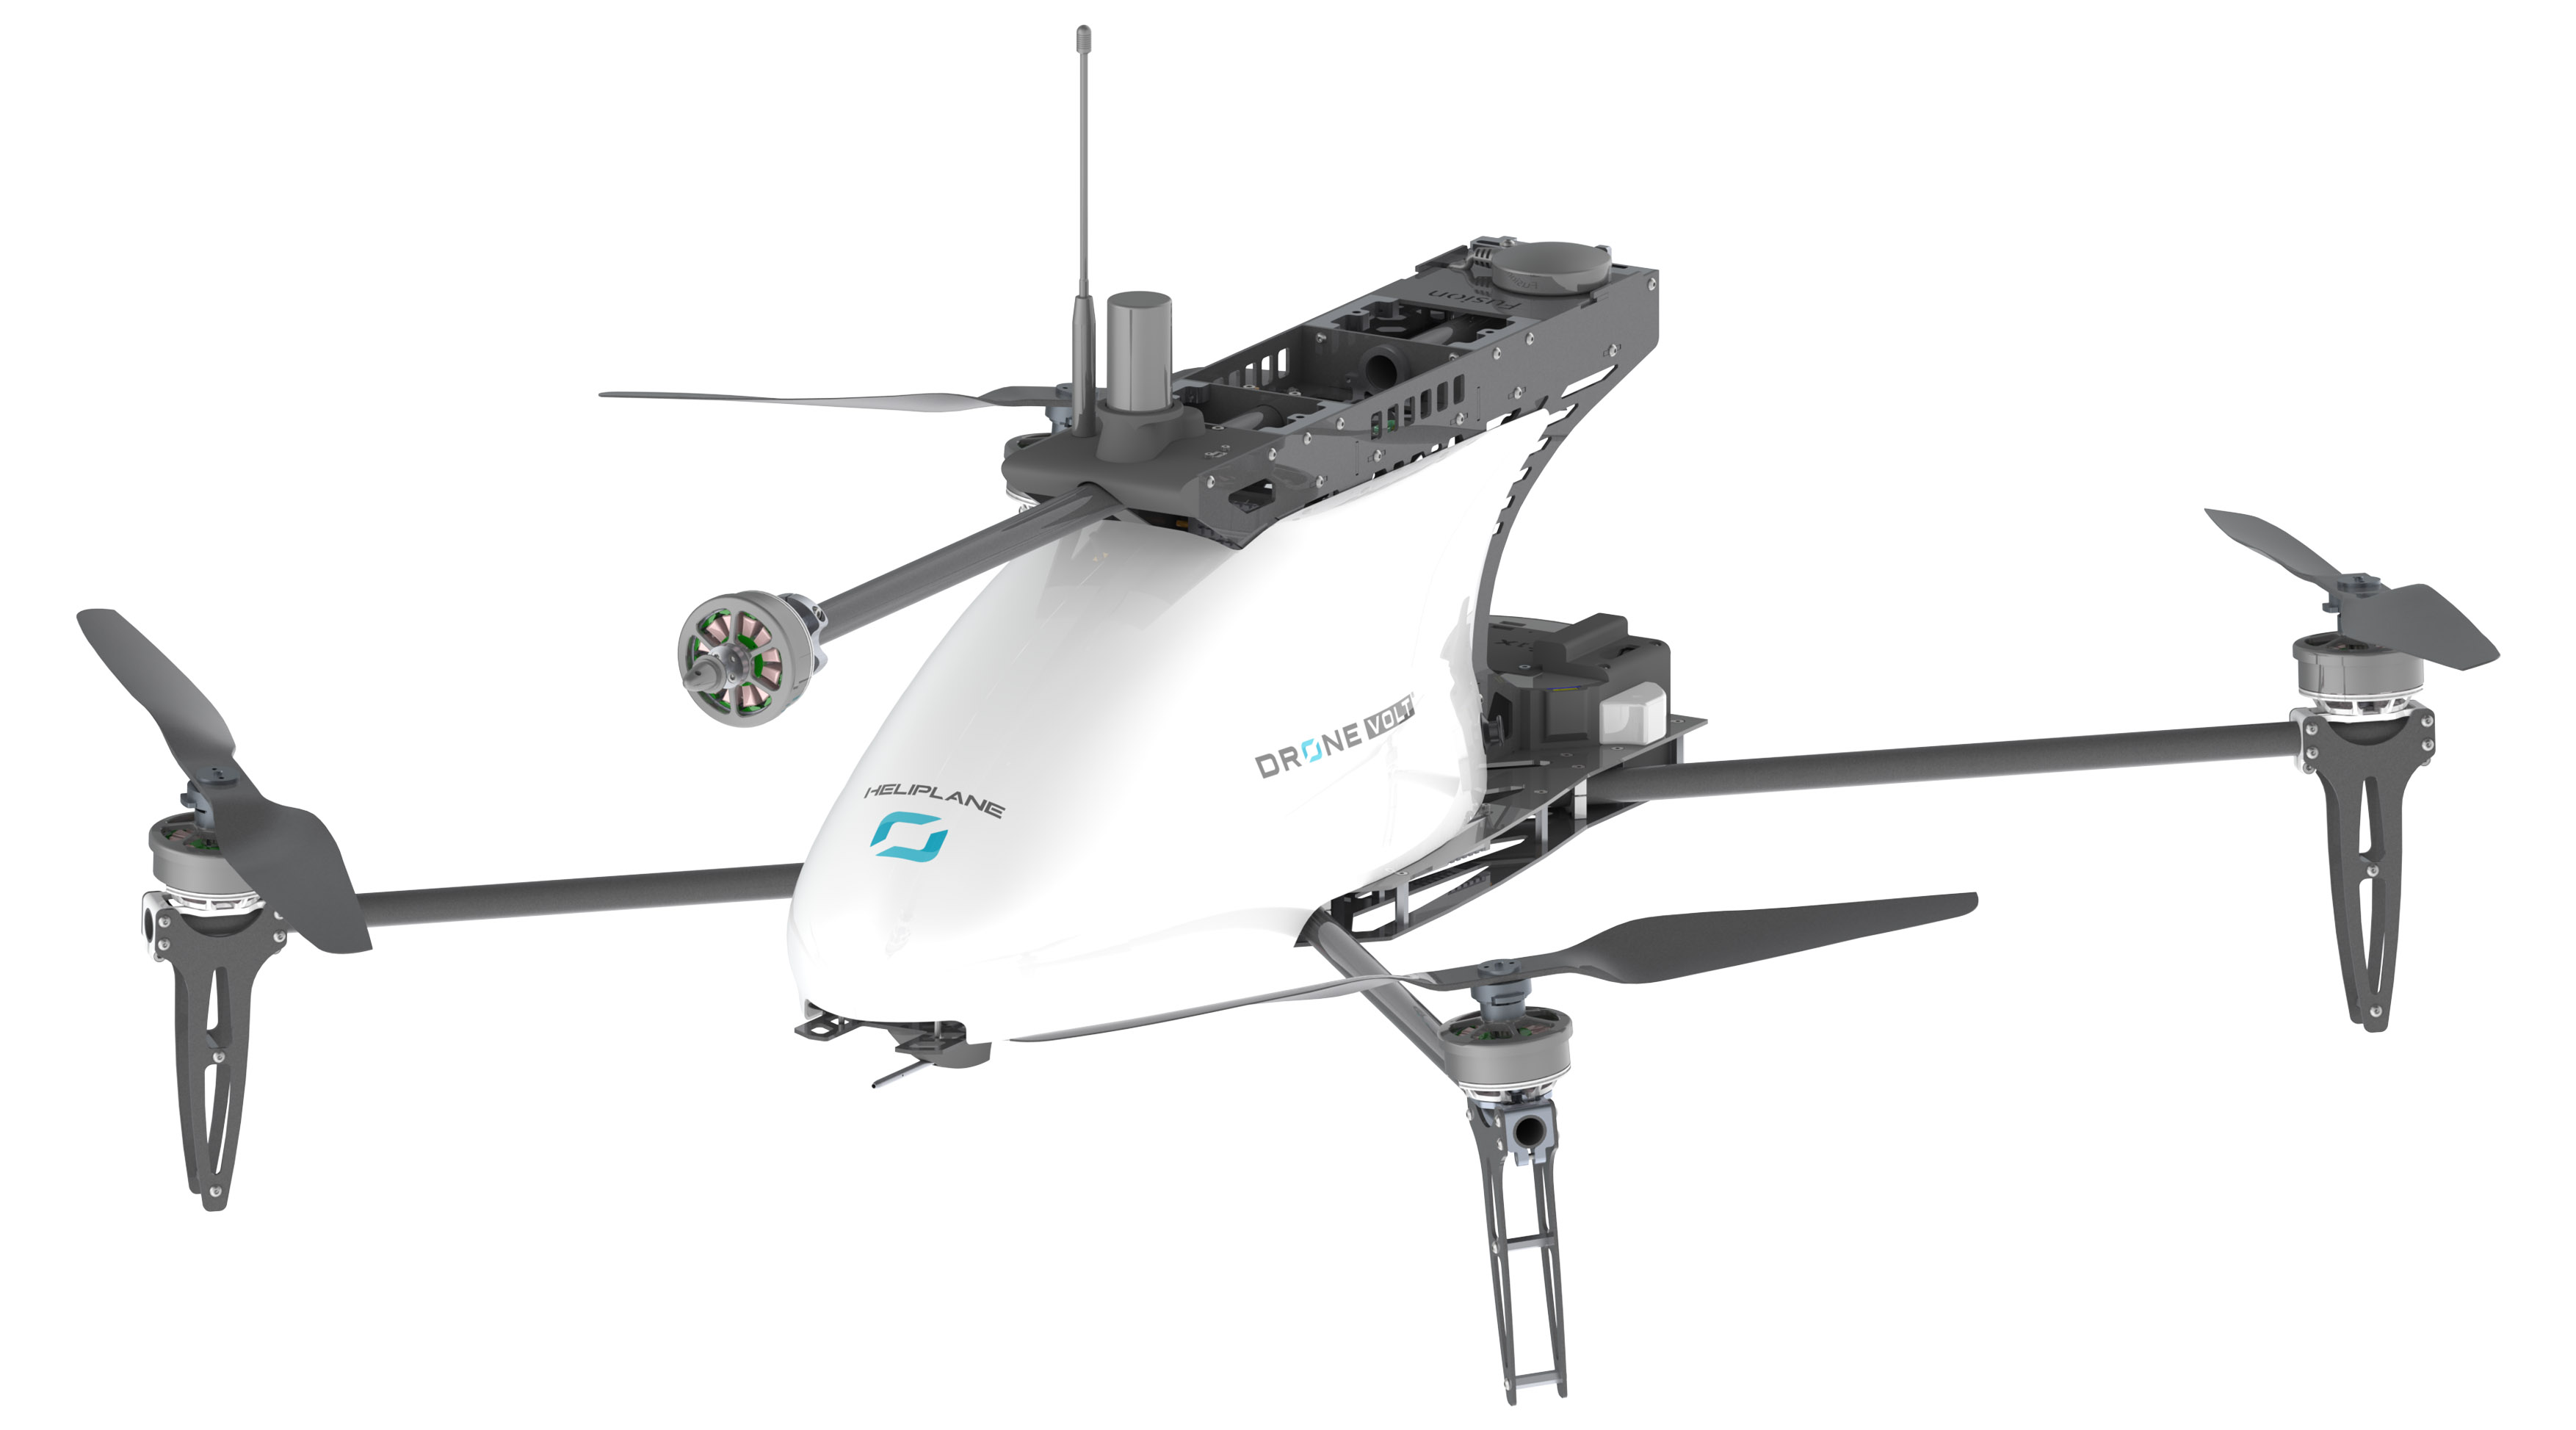
\includegraphics[width=\linewidth]{Images/Introduction/uav-multirotor-example.jpg}
        {(d) Multirotor} \URI{https://metatronus.com/heliplane/}
      \end{minipage}
      % -----------------
    \hfill \break
    \decoRule
    \caption[UAV Examples]{\Abbr{UAV} Examples}
    \label{fig:UAV-samples}
\end{figure}

Τυπικά τα Fixed-Wing drones είναι αρκετά ακριβά, χρειάζονται εξειδικευμένους χει\-ριστές για να λειτουργήσουν, όπως 
επιπλέον και περισσότερο χώρο για την απογείωση και την προσγείωση. Είναι ιδανικά για εφαρμογές που χρειάζεται να 
καλύψουμε μεγάλες περιοχές και συχνά έχουν αυτονομία τουλάχιστον μερικών ωρών. Για αυτούς τους λόγους χρησιμοποιούνται 
κυρίως από κυβερνήσεις, στρατιωτικές μονάδες ή επιχειρήσεις για την γρήγορη επίβλεψη μεγάλων εκτάσεων \cite{fixed-wing}.  

Τα Fixed-Wing Hybrid προσπαθούν να λύσουν τα μειονεκτήματα που έχουν τα Fixed-Wing drones, την μη ικανότητα δηλαδή για 
Vertically Hover, Take-off, and Land (\Abbr{VTOL}) όμως είναι ακόμα σε αρχικά στάδια
\cite{application-areas|swarm-types|uavs-classification|sensor's-used|swarms-problems|public-awareness}.

Τα Single Rotor είναι επίσης αρκετά ακριβά, πολύπλοκα μηχανολογικά μηχανήμα- τα, που δέχονται πολλούς κραδασμούς, 
απαιτούν εξειδικευμένους χειριστές όμως μπορούν να μεταφέρουν αρκετά βαριά payloads, θετικό στην χρήση τους ότι 
μπορούν να πραγματοποιήσουν \Abbr{VTOL} \cite{application-areas|swarm-types|uavs-classification|sensor's-used|swarms-problems|public-awareness}.

Τα Multirotor είναι ίσως τα πιο ευρέως διαδεδομένα. Καθώς είναι τα πιο οικονομικά από τα παραπάνω και εύκολο να κατασκευαστούν.
Πραγματοποιούν επίσης \Abbr{VTOL}, ενώ μπορούν να βρεθούν στο εμπόριο με διάφορο πλήθος από έλικες και είναι το κύριο είδος που 
χρησιμοποιείται από ερασιτέχνες ή χομπίστες για λόγους αναψυχής 
\cite{application-areas|swarm-types|uavs-classification|sensor's-used|swarms-problems|public-awareness}.

Στο \Fig{UAV-samples} δίνονται κάποια ενδεικτικά παραδείγματα \Abbr{UAV}<s> με βάση την κατηγοριοποίηση του \Tabl{drone-determined-by-their-structure}.
Φυσικά αυτή η κατηγοριοποίηση δεν περιλαμβάνει όλα τα είδη drone, είναι όμως ικανοποιητική για να γίνουν ξεκάθαρες δύο βασικές ιδέες. Αρχικά ανάλογα 
με την εφαρμογή που μας ενδιαφέρει, θα πρέπει να επιλέξουμε την χρήση του πλέον κατάλληλου τύπου drone. Όπως επίσης με βάση την επιλογή του 
συγκεκριμένου τύπου - αυτόματα έχουμε να διαχειριστούμε τα πλεονεκτήματα ή τα μειονεκτήματα που έχει.

Αυτά είναι και τα δύο σημεία στα οποία θα πρέπει να δοθεί ιδιαίτερη προσοχή στον σχεδιασμό του συστήματος που θα αναλυθεί στα επόμενα κεφάλαια.

Σε περίπτωση που μας ενδιαφέρει, οι συγγραφείς του \cite{drone-classification} παρουσιάζουν με εκτενέ\-στερο τρόπο, διάφορες κατηγοριοποιήσεις
και είδη drone τα οποία δεν εμπίπτουν στα πλαίσια αυτής της διπλωματικής και κυμαίνονται από smart dust, bio-drones, hybrid drones και άλλα πολλά.

%----------------------------------------------------------------------------------------
\subsection{Characteristics} \label{sec:Chapter1-1-2}
Σε όποια από τις κατηγορίες και αν αντιστοιχεί ένα drone
από την στιγμή που είναι ένα ιπτάμενο αντικείμενο, θα πρέπει να έχει την δυνατότητα να κινείται -
φυσικά - στον αέρα. Στο \Fig{UAV-principal-axes} παρουσιάζονται στους 3 άξονες, τα 6
Degrees of Freedom (\Abbr{DoF}) - τόσο \emph{Transitional} όσο και \emph{Rotational} - ενός \Abbr{UAV} \cite{aircraft-principal-axes} καθώς και το όνομα
που δίνεται στην κίνηση ανάλογα με τον άξονα που πραγματοποιείται.

% IMAGE
\FigCaptLabelBasedURL{Images/Introduction/aircraft-principal-axes.png}
{UAV principal axes}%
{UAV-principal-axes}%
<0.6>%
(http://www.chrobotics.com/library/understanding-euler-angles)

Ζούμε σε μία ψηφιακή εποχή, στην οποία ένα από τα πιο σημαντικά κατορθώματα είναι η ανάπτυξη των Integrated Circuits 
(\Abbr{IC}<s>) \& Μicro-electro-mechanical Sy\-stems (\Abbr{MEMS}) \cite{mems}, πράγμα το οποίο έχει βοηθήσει - έξυπνες 
συσκευές γεμάτες με αισθητήρες να βρίσκονται γύρω μας. Τέτοια τεχνολογικά επιτεύγματα όπως τα drones είναι συνεπώς εξοπλισμένα με 
Micro Controller Units (\Abbr{MCU}) \cite{mcu} ή Micro Processor Units (\Abbr{MPU}) \cite{mpu} για τον έλεγχο τους, ενώ δεν θα 
μπορούσαν να μην περιλαμβάνουν πλέον και ένα μεγάλο πλήθος και εύρος διαφορετικών τύπων sensors on-board. Με δύο από τους πιο σημαντικούς 
να είναι το Electronic Speed Control (\Abbr{ESC}) \cite{electronic-speed-control} και το Inertial Measurement Unit 
(\Abbr{IMU}) \cite{inertial-measurement-unit} - τα οποία χρησιμοποιούνται ώστε το drone να μπορεί να διατηρεί μία σταθερή και ελεγχόμενη πτήση
\cite{application-areas|swarm-types|uavs-classification|sensor's-used|swarms-problems|public-awareness}.
Εκτός από αυτούς βέβαια, ένα drone μπορεί να διαθέτει Global Positioning System (\Abbr{GPS}), camera για λήψη οπτικού υλικού ή ελέγχου μέσω 
First Person View (\Abbr{FPV}), Obstacle avoidance sensors ή ακόμα και άλλους. Με κύριο περιορισμό\udot τα αισθητήρια όργανα να βρίσκονται στο 
εύρος βάρος του payload, που μπορεί να μεταφέρει το drone. 

Σε αυτό το section πραγματοποιήθηκε μία πρώτη οριοθέτηση του όρου drone, παρόλα αυτά
δεν αναφέρθηκαν λόγοι ύπαρξης τους, καθώς και εφαρμογές τους.  Η ύπαρξης των swarms είναι ουσιαστικά η 
κάλυψη των αναγκών από των individual drones σε μεγαλύτερη κλίμακα, για αυτό\udot μερικές από τις εφαρμογές των drone - βρίσκονται
στο \Sect{Chapter1-2-2}.


%----------------------------------------------------------------------------------------
%	SECTION 2
%----------------------------------------------------------------------------------------
\section{Motivation} \label{sec:Chapter1-2} 
Ξεκινώντας από τα individual drones, αξίζει να σημειωθεί ότι το  \href{https://www.tuc.gr/}{Πολυτεχνείο Κρήτης} έχει ένα ενεργό
ερευνητικό ιστορικό στον τομέα των αεροχημάτων. Το SenseLab στο οποίο υπεύθυνος καθηγητής είναι ο κύριος
Παρτσινέβελος της Σχολής Μηχανικών Ορυκτών Πόρων να είναι ένα από αυτά -
και μάλιστα με πολλαπλές διακρίσεις  σε διεθνείς διαγωνισμούς \cite{senselab-demo} \cite{senselab-site}. 

%-----------------------------------------------------------------------------------
\subsection{Nature} \label{sec:Chapter1-2-1}
Στην φύση είναι αρκετά συχνή η ύπαρξη έμβιων οργανισμός που κινούνται σε ομάδες, με μερικά από αυτά ως παράδειγμα, τα σμήνη από πουλιά και
έντομα, κοπάδια ψαριών ή και αγέλες ζώων. Σκοπός της συνεργασίας τους είναι κυρίως η προστασία από θηρευτές ή άλλοι σχετικοί με την επιβίωση.
Αρκετές έρευνες έχουν γίνει εμπνευ\-σμένες σε αυτό, ακόμα και στον τομέα των fleet of drones
\cite{research-on-drone-swarms-move-like-animals} \cite{research-on-drone-swarms-move-like-animals-like-documentary} \cite{swarm-of-drones}.
  
%-----------------------------------------------------------------------------------
\subsection{Swarms and Applications} \label{sec:Chapter1-2-2}
Από μόνο του ένα {\Abbr{UAV} σε πολλές περιπτώσεις θα μπορέσει να φέρει εις πέραν την αποστολή 
που του έχει ανατεθεί. Πολύ εύκολα όμως μπορούν να δημιουργηθούν ζητήματα αξιοπιστίας, όταν ένα μεμονωμένο drone
χρειάζεται ως παράδειγμα να χα\-ρτογραφήσει σε μικρό χρονικό διάστημα ένα άγνωστο και μεγάλης έκτασης περιβάλλον. Όπως επίσης, εάν θα θέλαμε να
διαθέτει πολλαπλούς αισθητήρες για να έχουμε πιο λεπτομερείς δεδομένα σε μία αποστολή, όμως αυτό να είναι αδύνατον διότι 
υπε\-ρβαίνουν το δυνατόν payload που μπορεί να μεταφέρει
το drone. Η ακόμα, και για το ενδεχόμενο αποτυχίας της αποστολής, σε κάποιο πιθανό malfunction που θα πραγματοποιηθεί στο ιπτάμενου όχημα.
Μπορούμε να πούμε λοιπόν\udot σε μία abstract σύγκριση με αυτή των ζώων, ότι ωθούμαστε για ανάλογους σκοπούς στην χρήση των swarms ώστε
να ξεπεράσουμε αυτά τα προβλήματα \cite{reason-for-working-together|related-swarm-research}.  

Με τον όρο Swarm Robotics (\Abbr{SR}) συχνά αναφερόμαστε στην μεθοδολογία που ακολουθούμε ώστε να συντονίζουμε πολλαπλές 
ανεξάρτητες ρομποτικές οντότητες να συμπεριφέρονται συνεργατικά\udot ως ένα ενιαίο σύστημα \cite{what-is-swarm-robotics}.
Με τον όρο συνε\-ργα\-τι\-κά, αυτό σημαίνει είτε να μπορούν να κινηθούν ως ομάδα \cite{moving-models-for-robotic-swarms}
\cite{swarm-formation-translation-rotation-attack-demo} \cite{lab-demo-of-formations-in-3d-movement-with-obstacles},
είτε να επικοινωνούν ώστε γνώση πληροφορίας την οποία έχει συλλέξει ένα από αυτά να μεταδίδεται
και στα υπόλοιπα (π.χ. σε περίπτωση που θέλουμε να κάνουμε 3D reconstruction μίας περιοχής ή γνώση της θέσης από 
την οποία λαμβάνεται - με χρήση της κάμερας - υλικό είναι σημαντική για την δημιουργία του ψηφιακού μοντέλου 
\cite{localization-importance-for-3d-scene-reconstruction}). 

Σήμερα τα drones καθώς και τα fleet of drones χρησιμοποιούνται σε ένα μεγάλος εύρος εφαρμογών.
Έχει γίνει αναφορά είδη από την αρχή του chapter ότι χρησιμοποιούνται για λόγους αναψυχής,
με μερικά παραδείγματα, την διεκπεραίωση shows \cite{intel's-shows-around-the-world-and-2018-drones-record}
\cite{ford's-100-drone-show} \cite{swarm-magic-show} και την καταγραφή οπτικού υλικού για δημιουργία 
ταινιών \cite{drones-for-filmmaking}. Άλλες πιο ζωτικής σημασίας χρήσεις τους, είναι σχετικές με 
environment mapping \cite{drones-enviroment-mapping}, police surveillance \cite{drones-police}, natural disaster inspection 
\cite{drones-natural-disaster},  Search \& Rescue (\Abbr{SandR}(S\symbol{`\&}R)) \cite{drones-for-search-and-rescue}, 
light cargo transportation \cite{drones-delivery} και πολλές άλλες. Ακόμα και στρατιωτικές επιχειρήσεις 
χρησιμοποιούν drones. Συνήθως σε αυτές τις περιπτώσεις αναφερόμαστε στην χρήση Unmanned Combat Aerial Vehicle (\Abbr{UCAV}) 
\cite{UCAVs} \cite{military-robots-samples-and-photos} και πολλές από τις εφα\-ρμογές στο συγκεκριμένο
τομέα έχουν να κάνουν με Intelligence Surveillance, and Reconnaissance (\Abbr{ISR})
\cite{drones-isr}.

Για περισσότερες εφαρμογές των drones/swarms \cite{list-of-uav-applications} ή λεπτομέρειες σχετικά με αυτές, μπορούμε να ανατρέξουμε στην υφιστάμενη βιβλιογραφία 
\cite{application-senarios|related-work|the-platform-they-used|communication-infrastructure-and-problems}
\cite{some-applications} \cite{swarm-friendly-communications|brain-sensor-drones|different-swarm-applications|}.

%----------------------------------------------------------------------------------------
%	SECTION 3
%----------------------------------------------------------------------------------------
\section{Scientific Goals and Contributions} \label{sec:Chapter1-3} 
Όπως μπορεί να γίνει εύκολα αντιληπτό\udot η γνώση της σχετικής θέσης ενός {\Abbr{UAV} σε σχέση με τα υπόλοιπα του σμήνους, είτε σε συνδυασμό
αυτής σε απόλυτο τρόπο με βάση ένα καθορισμένο σύστημα αξόνων, 
είτε ακόμα και ο υπολογισμός της θέσης επιπλέον αντικειμένων - ενδιάμεσα του σμήνους - τα οποία σχετίζονται με την ε\-κά\-στο\-τε αποστολή,
είναι αρκετά σημαντική για ένα πολύ μεγάλο πλήθος εφαρμογών.
Σκοπός της συγκεκριμένης διπλωματικής εργασίας, είναι να γίνει η απαραίτητη ε\-ρευ\-νη\-τι\-κή
αναζήτηση, ώστε να επιτευχθεί ο σχεδιασμός καθώς και η υλοποίηση ενός ενσωματωμένου συστήματος - το 
οποίο να είναι σε θέση με όσο το δυνατόν πιο οικονομικό τρόπο - να υπολογίζει την θέση αντικειμένων από drone όταν αυτά πετούν σε σχηματισμό, το ακριβές 
πρόβλημα το οποίο θα γίνει προσπάθεια να επιλυθεί καθώς και η μεθοδολογία, παρουσιάζονται αναλυτικά στο Chapter \ref{chap:thesis-approach}.  

%----------------------------------------------------------------------------------------
%	SECTION 4
%----------------------------------------------------------------------------------------
\section{Thesis Outline} \label{sec:Chapter1-4} 
    \begin{itemize}
        \item \textbf{Chapter \ref{chap:Chapter2} - {\hypersetup{hidelinks}\nameref{chap:Chapter2}}:} 
        Στην συγκεκριμένη ενότητα γίνεται μία συ\-νο\-πτική αναφορά σε τεχνικές που χρησιμοποιούνται ήδη, σύμφωνα με την βιβλιο\-γραφία,
        για την εύρεσης θέσης σχετιζόμενα με drone.  
        \item \textbf{Chapter \ref{chap:Chapter3} - {\hypersetup{hidelinks}\nameref{chap:Chapter3}}:}
        Σε αυτό το κεφάλαιο παρουσιάζεται το απαραίτητο μαθηματικό υπόβαθρο, καθώς και βασικές μεθοδολογίες εύρεσης τοποθεσία, 
        που προέρχονται από ευρύτερους τομείς, όπως των Wireless Sensor Networks (\Abbr{WSN}).
        \item \textbf{Chapter \ref{chap:Chapter4} - {\hypersetup{hidelinks}\nameref{chap:Chapter4}}:}
        Σε αυτό το σημείο παρουσιάζεται η διαδικασία σχεδιασμού του ενσωματωμένου συστήματος που σχετίζεται αυτή η διπλωματική.
        % \item \textbf{Chapter \ref{chap:Chapter5} - {\hypersetup{hidelinks}\nameref{chap:Chapter5}}:}       %Maybe rename chapter's name
        % TODO:
        \item \textbf{Chapter \ref{chap:Chapter6} - {\hypersetup{hidelinks}\nameref{chap:Chapter6}}:}
        Στο παρόν κεφάλαιο παρουσιάζονται οι απαραίτητοι έλεγχοι που έγιναν για την επαλήθευση της ορθής λειτουργίας του συστήματος.
        \item \textbf{Chapter \ref{chap:Chapter7} - {\hypersetup{hidelinks}\nameref{chap:Chapter7}}:} 
        Στο συγκεκριμένο κεφάλαιο παρουσιάζονται τα τελικά συμπεράσματα τα οποία βγήκαν από το σύνολο της διπλωματικής - 
        καθώς και κάποιες από τις πιθανές μελλοντικές εξελίξεις της.
    \end{itemize}
